\documentclass{article}
\usepackage[margin=1in]{geometry}
\usepackage{tikz}
\usetikzlibrary{positioning,arrows.meta,shapes.geometric}
\usepackage{tcolorbox}
\usepackage{fontawesome5}
\usepackage{xcolor}

\newcommand{\benchmark}{ChemChain}

\begin{document}

\begin{figure}[t]
    \centering

    % VERSION 1: Hierarchical Flow Layout
    \begin{tcolorbox}[
        title=\textbf{Chemistry: Reaction Cascade} \hfill {\small\colorbox{teal!20}{Medium} \quad 9 steps},
        colframe=teal!70!black,
        colback=teal!3,
        boxrule=0.8pt,
        width=\textwidth
    ]
    \small
    \begin{tikzpicture}[remember picture, overlay]
        \node[opacity=0.06, anchor=east] at ([xshift=-0.5cm, yshift=0.3cm]current page.east) {\Huge\faFlask};
    \end{tikzpicture}

    \textbf{Dependency graph:}
    \begin{center}
    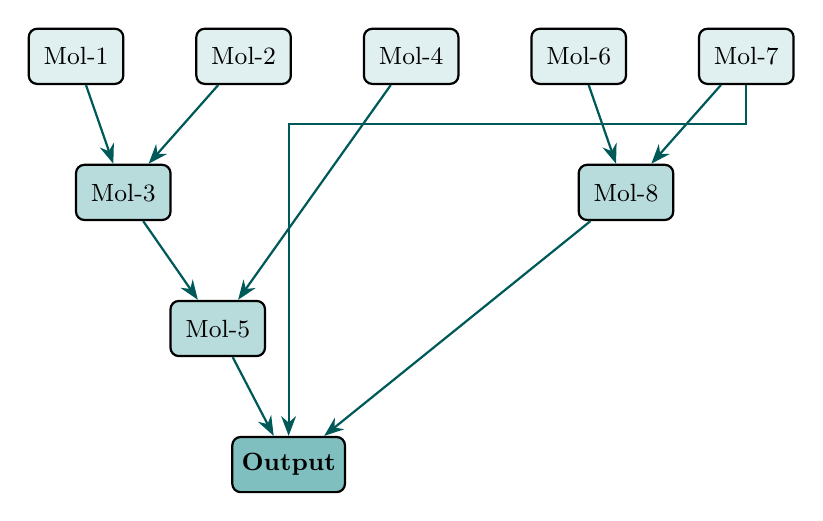
\begin{tikzpicture}[
        node distance=1.2cm and 0.9cm,
        every node/.style={font=\small},
        mol/.style={draw, rounded corners=3pt, minimum width=1.2cm, minimum height=0.7cm, thick},
        input/.style={mol, fill=teal!12},
        intermediate/.style={mol, fill=teal!28},
        output/.style={mol, fill=teal!50, font=\small\bfseries},
        arrow/.style={-{Stealth[length=2.5mm]}, thick, teal!70!black}
    ]
        % Layer 1: Inputs
        \node[input] (m1) {Mol-1};
        \node[input, right=of m1] (m2) {Mol-2};
        \node[input, right=of m2] (m4) {Mol-4};
        \node[input, right=of m4] (m6) {Mol-6};
        \node[input, right=of m6] (m7) {Mol-7};

        % Layer 2: First intermediates
        \node[intermediate, below=1.0cm of m1.south, xshift=0.6cm] (m3) {Mol-3};
        \node[intermediate, below=1.0cm of m6.south, xshift=0.6cm] (m8) {Mol-8};

        % Layer 3: Second intermediate
        \node[intermediate, below=1.0cm of m3.south, xshift=1.2cm] (m5) {Mol-5};

        % Layer 4: Output
        \node[output, below=1.0cm of m5.south, xshift=0.9cm] (out) {Output};

        % Arrows with slight curves for clarity
        \draw[arrow] (m1) -- (m3);
        \draw[arrow] (m2) -- (m3);
        \draw[arrow] (m3) -- (m5);
        \draw[arrow] (m4) -- (m5);
        \draw[arrow] (m6) -- (m8);
        \draw[arrow] (m7) -- (m8);
        \draw[arrow] (m5) -- (out);
        \draw[arrow] (m7) |- ([yshift=-0.5cm]m7.south) -| (out);
        \draw[arrow] (m8) -- (out);
    \end{tikzpicture}
    \end{center}

    \vspace{0.1cm}
    \begin{tabular}{@{}p{0.48\textwidth}p{0.48\textwidth}@{}}
    \textit{Sample step (Subproblem 3):} React Mol-1 + Mol-2 in THF at room temp. Predict major product. &
    \textit{Final step:} Count hydrogens in Mol-5, Mol-7, Mol-8. \\
    \end{tabular}

    \vspace{0.25cm}
    \hfill \textbf{Answer:} \texttt{[19, 15, 23]}
    \end{tcolorbox}

    \caption{\textbf{Version 1:} Hierarchical flow layout with clear layers showing the reaction cascade from inputs (top) through intermediates to output (bottom). Lighter colors indicate input molecules, darker colors show reaction products.}
\end{figure}

\end{document}
